\documentclass{article}
\usepackage{graphicx}
\usepackage{siunitx} % Required for alignments
\begin{document}
	\title{GST 108: Quantitative Reasoning}

	\author{Ariyibi Joseph Iseoluwa}
\maketitle
\newpage
\tableofcontents
\newpage
\centering
\section{INTRODUCTION}
    A logic gate is a building block of a digital circuit which is at the heart of any computer operation.
    
   
   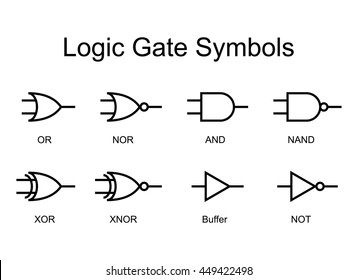
\includegraphics[width=1\linewidth]{logic}

	\subsection{Logic Gates}
		Logic gates perform logical operations that take binary input (0s and 1s) and produce a single binary output. They are used in most electronic device including:
	\begin{table}[h!]
		\begin{center}
			\caption{Logic Gates}
			\label{tab:table1}
			\begin{tabular}{l|c|c|}
				\hline
				Smartphones
				&
				Tablets
				&
				Memory Devices
				\\
				\hline
				
\includegraphics[width=0.2\linewidth]{iphone13}
				&
				
\includegraphics[width=0.25\linewidth]{ipadmini}
				&
				
\includegraphics[width=0.2\linewidth]{download}
				\\
				\hline
			\end{tabular}
		\end{center}
	\end{table}
\newpage
\section{Definition Of a Gate}
A gate is a basic electronic circuit which operates on one or more signals to produce an output signal. 
Logic gates are digital circuits constructed from diodes, transistors, and resistors connected in such a way that the circuit output is the result of a basic logic operation (OR, AND, NOT) performed on the inputs. \cite{okoacha2021logic}
\section{Types Of Logic Gates}
\textbf{Fundamental Gates include AND, OR, NOT gates}

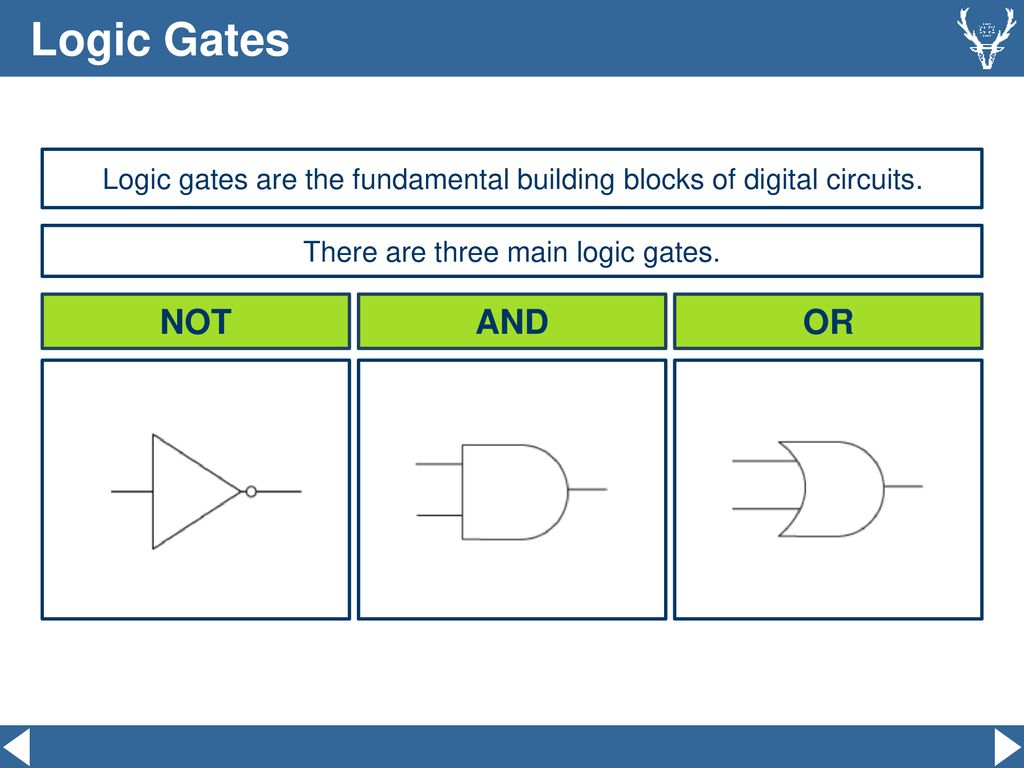
\includegraphics[width=1\linewidth]{gates.jpg}
\newpage
\subsection{AND Gate}

The expression C = A X B reads as “C equals A AND B“ 
The multiplication sign (X) stands for the AND operation, same for ordinary multiplication of 1s and 0s.
The AND operation produces a true output (result of 1) only for the single case when all of the input variables are 1 and a false output (result of 0) where one or more inputs are 0.

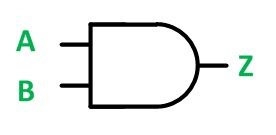
\includegraphics[width=0.3\linewidth]{and.jpg}
\begin{table}[h!]
	\begin{center}
		\caption{AND TABLE}
		\begin{tabular}{c|c|c|}
			\textbf{A} & \textbf{B} &  \textbf{C= A x B} \\
			\hline
			\textbf{1} & \textbf{1} & \textbf{1} \\
			\textbf{1} & \textbf{0} & \textbf{0} \\
			\textbf{0} & \textbf{1} & \textbf{0} \\
			\textbf{0} & \textbf{0} & \textbf{0} \\
		\end{tabular}
	\end{center}
\end{table}
\subsection{OR GATE}
The expression C = A + B reads as “C equals A OR B". It is the inclusive “OR”
The Addition (+) sign stands for the OR operation.
The OR operation produces a true output (result of 1) when any of the input variable is 1 and a false output (result of 0) only when all the input variables are 0.
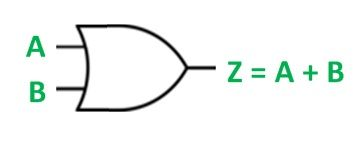
\includegraphics[width=0.6\linewidth]{or.jpg}
\begin{table}
	\begin{center}
		\caption{OR TABLE}
		\begin{tabular}{l|c|c|}
			\textbf{A} & \textbf{B} & \textbf{C= A + B} \\
			\hline
			\textbf{1} & \textbf{1} & \textbf{1} \\
			\textbf{1} & \textbf{0} & \textbf{1} \\
			\textbf{0} & \textbf{1} & \textbf{1} \\
			\textbf{0} & \textbf{0} & \textbf{0} \\
		\end{tabular}
	\end{center}
\end{table}
\newpage
\subsection{NOT GATE}
The NOT gate is called a logical inverter.
It has only one input. It reverses the original input (A) to give an inverted output C.
C = NOT A or C = $\overline{A}$
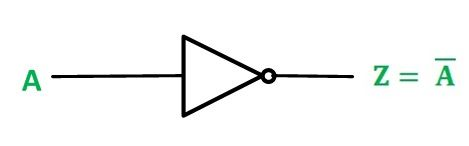
\includegraphics[width=0.6\linewidth]{not.jpg}

\begin{table}[h!]
	\begin{center}
		\caption{NOT TABLE}
		\begin{tabular}{c|c|}
			\textbf{A} & \textbf{C = $\overline{A}$} \\
			\hline
			\textbf{1} & \textbf{0} \\
			\textbf{0} & \textbf{1} \\
		\end{tabular}
	\end{center}
\end{table}
\subsection{NOR GATE}
The NOR (NOT OR) gate circuit is an inverter OR gate

C =  $\overline{(A + B)}$
Reads as C = NOT of A or B
 
The NOR Gate gives a true output (result of 1) only when both inputs are false (0)

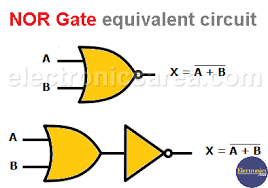
\includegraphics[width=0.6\linewidth]{nor}
\begin{table}[h!]
	\begin{center}
		\caption{NOR TABLE}
		\begin{tabular}{l|c|c|c|}
			\textbf{A} & \textbf{B} & \textbf{A+B} & \textbf{C= (A+B)} \\
			\hline
			\textbf{1} & \textbf{1} & \textbf{1} & \textbf{0} \\
			\textbf{1} & \textbf{0} & \textbf{1} & \textbf{0} \\
			\textbf{0} & \textbf{1} & \textbf{1} & \textbf{0} \\
			\textbf{0} & \textbf{0} & \textbf{0} & \textbf{1} \\
		\end{tabular}
	\end{center}
\end{table}
\newpage
\subsection{NAND GATE}
The NAND (NOT AND) Gate is an inverted AND Gate
C = ($\overline{(A * B)}$) 
Reads as C = NOT of A AND B
The NAND Gate gives a false output (result of 0) only when both inputs are true (1)

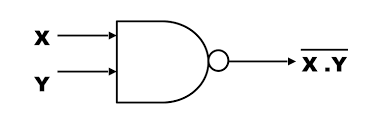
\includegraphics[width=0.7\linewidth]{nand}
\begin{table}[h!]
	\begin{center}
		\caption{NAND GATE}
		\begin{tabular}{l|c|c|c|}
			\textbf{A} & \textbf{B} & \textbf{A x B} & \textbf{C= $\overline{(A * B)}$} \\
			\hline
			\textbf{1} & \textbf{1} & \textbf{1} & \textbf{0} \\
			\textbf{1} & \textbf{0} & \textbf{0} & \textbf{1} \\
			\textbf{0} & \textbf{1} & \textbf{0} & \textbf{1} \\
			\textbf{0} & \textbf{0} & \textbf{0} & \textbf{1} \\
		\end{tabular}
	\end{center}
\end{table}

The NAND Gate is a universal gate because it can be used to form any other kind of gate 
\newpage
\subsection{XOR GATE}
An XOR (exclusive OR) gate acts in the same way as the exclusive OR logical connector. 
It gives a true output (result of 1) if one, and only one, of the inputs to the gate is true (1), i.e either or but not both

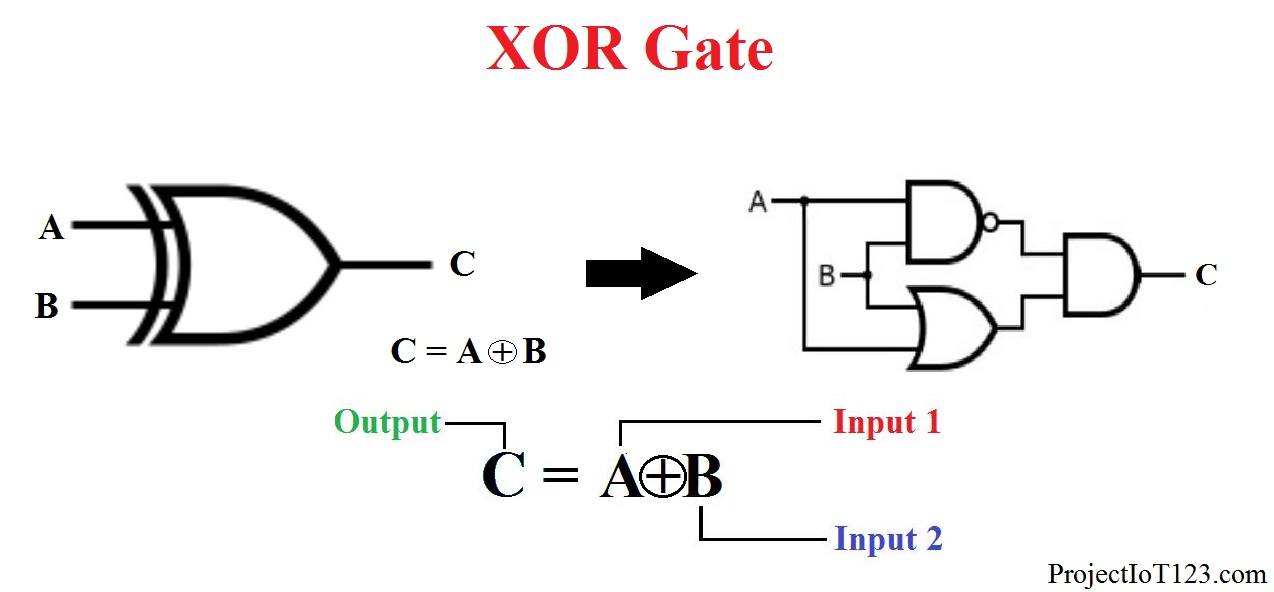
\includegraphics[width=0.7\linewidth]{xor}
\begin{table}[h!]
 \begin{center}
 	\caption{XOR GATE}
 	\begin{tabular}{l|c|c|c|c|c|c|}
 		\textbf{A} & \textbf{B} & \textbf{$\overline{A}$} & \textbf{$\overline{B}$} & \textbf{$\overline{A}$.B} & \textbf{$\overline{B}$.A} & \textbf{$\overline{A}$.B + $\overline{B}$.A} \\
 		\hline
 		\textbf{1} & \textbf{1} & \textbf{0} & \textbf{0} & \textbf{0} & \textbf{0} & \textbf{0} \\
 		\textbf{1} & \textbf{0} & \textbf{0} & \textbf{1} & \textbf{0} & \textbf{1} & \textbf{1} \\
 		\textbf{0} & \textbf{1} & \textbf{1} & \textbf{0} & \textbf{1} & \textbf{0} & \textbf{1} \\
 		\textbf{0} & \textbf{0} & \textbf{1} & \textbf{1} & \textbf{0} & \textbf{0} & \textbf{0}
 	\end{tabular}
 \end{center}
\end{table}
\newpage
\subsection{XNOR GATE}
The XNOR (exclusive - NOR) gate is a combination XOR gate followed by an inverter. It is represented by the $\odot$
Its gives a  true output (1), if the inputs are the same, and a false output (0) if the inputs are different. 

C = $\overline{(A \odot B)}$ =$\overline{\overline{A} .B + \overline{B} .A}$
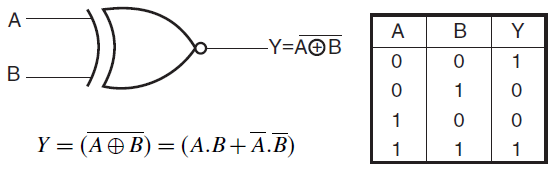
\includegraphics[width=0.7\linewidth]{xnor}
\begin{table}[h!]
	\begin{center}
		\caption{XNOR GATE}
		\begin{tabular}{l|c|c|c|c|c|c|c|}
			\textbf{A} & \textbf{B} & \textbf{$\overline{A}$} & $\overline{B}$ & \textbf{$\overline{A}$ .B} & \textbf{$\overline{B}$ .A} & \textbf{$\overline{A}$ .B + $\overline{B}$ .A} & \textbf{$\overline{\overline{A} .B + \overline{B} .A}$} \\
			\hline
			\textbf{1} & \textbf{1} & \textbf{0} & \textbf{0} & \textbf{0} & \textbf{0} & \textbf{0} & \textbf{1} \\
			\textbf{1} & \textbf{0} & \textbf{0} & \textbf{1} & \textbf{0} & \textbf{1} & \textbf{1} & \textbf{0} \\
			\textbf{0} & \textbf{1} & \textbf{1} & \textbf{0} & \textbf{1} & \textbf{0} & \textbf{1} & \textbf{0} \\
			\textbf{0} & \textbf{0} & \textbf{1} & \textbf{1} & \textbf{0} & \textbf{0} & \textbf{0} & \textbf{1} \\
		\end{tabular}
	\end{center}
\end{table}
\newpage
\section{Summary}
\subsection{LOGIC GATES AND THEIR TRUTH TABLE}
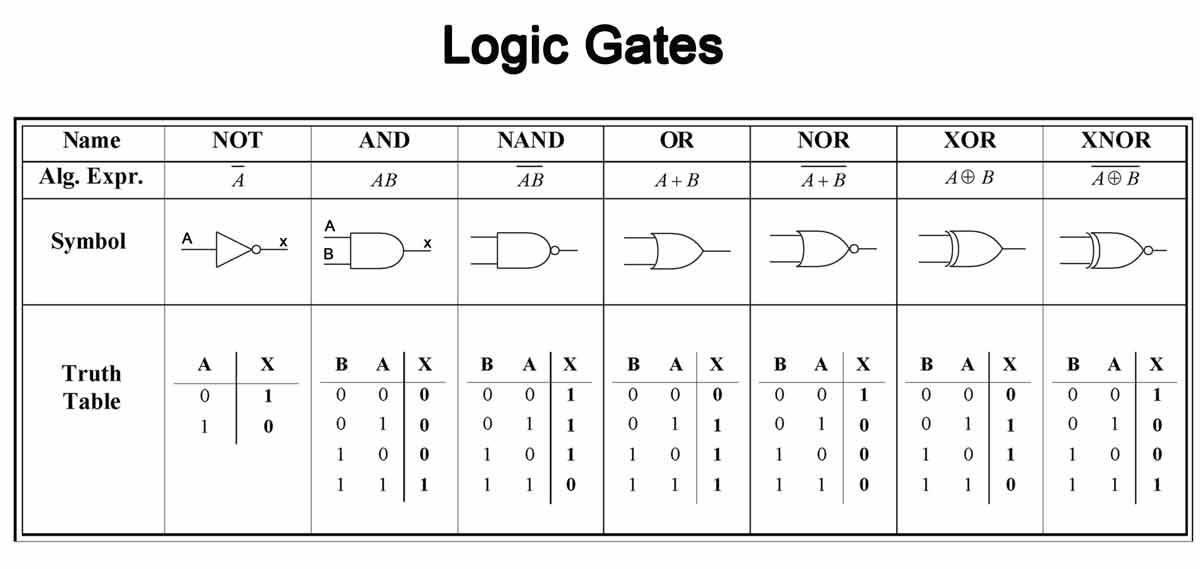
\includegraphics[width=0.8\linewidth]{truth table}
\subsection{Summary contd.}
Using different combination of logic gates, complex operations can be performed. 
With the Universal logic gates - NAND and NOR, any other gate can be built.

There is no limit to the number of gates that can be arranged together in a single device.  
However, in practice, there is a limit to the number of gates that can be packed into a given physical space. 
Arrays of logic gates are found in digital integrated circuits.
The logic gates are abstract representations of real electronic circuits. \cite{okoacha2021sum}

In computers, Logic gates are built using transistors combined with other electrical components like resistors and diodes. 
These electrical components are wired together in order to transform a particular input to give a desired output.
\newpage
\section{QUIZ}
\begin{enumerate}
\item	What is the output of an AND gate if the inputs are 1 and 0?
	
\item	Explain the difference between the AND gate and the OR gate.
	
\item	What is the output of a NOT gate if the inputs is 0?
	
\item	Which logic gate is this?
\begin{center}
	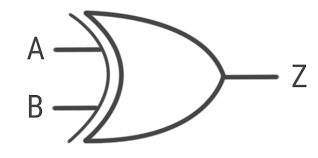
\includegraphics[width=0.6\linewidth]{xor2}
\end{center}
	
\item	Which gate is also known a logical converter?
	
\end{enumerate}
\newpage
\bibliography{gst}
\bibliographystyle{ieeetr}
\end{document}
